\documentclass[a4paper,11pt]{article}

\usepackage[english]{babel}
\usepackage[utf8]{inputenc}
\usepackage[vmargin=3.5cm,hmargin=2cm]{geometry}
\usepackage{graphicx}
\usepackage{caption}
\usepackage{subcaption}
\usepackage{amsmath}
\usepackage{mathtools}
\usepackage{fancyhdr}
\usepackage{listings}
\usepackage{makeidx}

\setlength{\footskip}{0cm}
\setlength\parindent{0pt}
\addtolength{\footskip}{0.8cm}
\addtolength{\headsep}{-.5cm}

\title{\bfseries Lab 2 \\}
\date{}

\lfoot{}
\cfoot{}
\rfoot{\textbf{Communication Systems} \\ Teresa Algarra Ulierte }

\renewcommand{\headrulewidth}{0.5pt}
\renewcommand{\footrulewidth}{0.5pt}

\begin{document}
\renewcommand\contentsname{\vspace{-1cm}}
\maketitle
\lstset{language=Matlab}

\begin{centering}
    Teresa Algarra Ulierte \\
    Student ID: teresaalgarraulierte \\
    Perm number: 7626872 \\
\end{centering}

\vspace{3cm}

\begin{figure}[!ht]
	\centering
	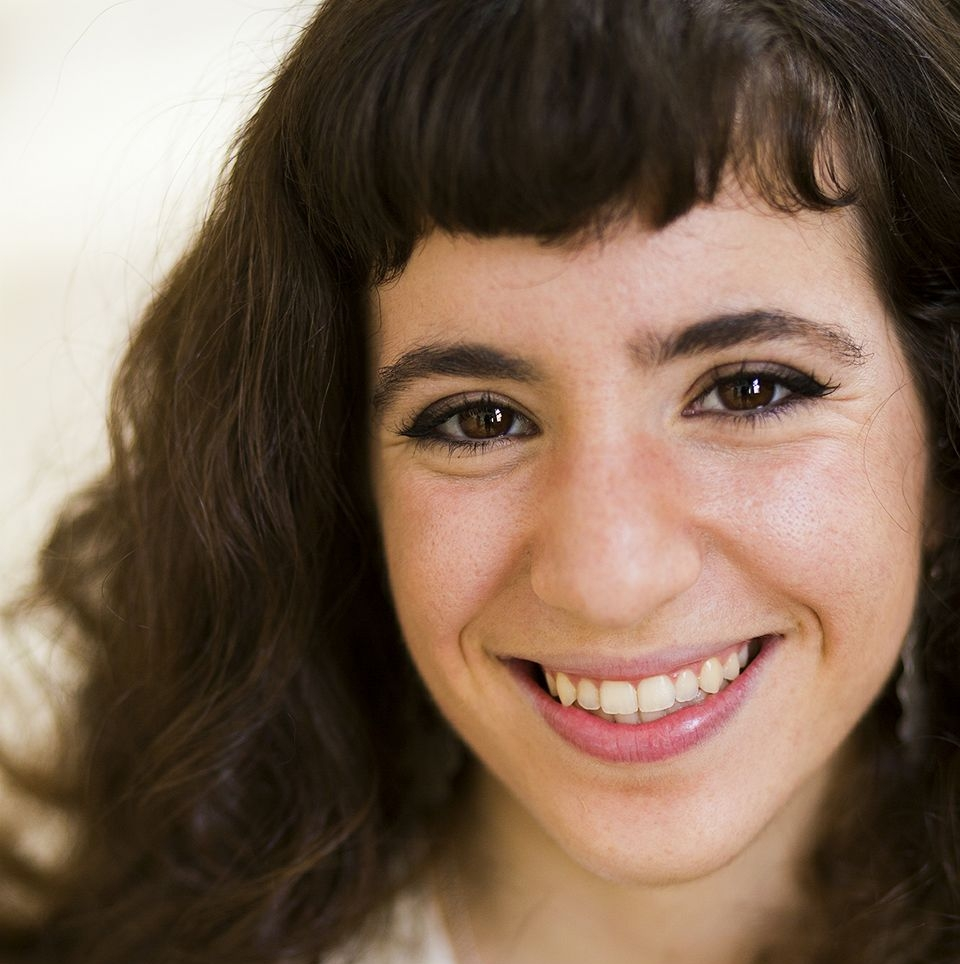
\includegraphics[scale = 0.25]{images/photo.jpg}
\end{figure}

\newpage

\section{Lab 2.2: Modeling Carrier Phase Uncertainty}

\subsection{Goal of the lab:}

The goal of this lab is to illustrate how wireless multipath channels can be
modeled in complex baseband.

\subsection{Laboratory assignment:}

\newpage

\section{Lab 2.3: Modeling a Lamppost based Broadband Network}

\subsection{Goal of the lab:}

The goal of this lab is to illustrate how wireless multipath channels can be
modeled in complex baseband, that is, the same as Lab 2.2.

\subsection{Laboratory assignment:}

\vspace{4cm}

\end{document}
